\chapter{Design}
\label{sec:design}

% Ist das zentrale Kapitel der Arbeit. Hier werden das Ziel sowie die
% eigenen Ideen, Wertungen, Entwurfsentscheidungen vorgebracht. Es kann
% sich lohnen, verschiedene Möglichkeiten durchzuspielen und dann
% explizit zu begründen, warum man sich für eine bestimmte entschieden
% hat. Dieses Kapitel sollte - zumindest in Stichworten - schon bei den
% ersten Festlegungen eines Entwurfs skizziert werden.
% Es wird sich aber in einer normal verlaufenden
% Arbeit dauernd etwas daran ändern. Das Kapitel darf nicht zu
% detailliert werden, sonst langweilt sich der Leser. Es ist sehr
% wichtig, das richtige Abstraktionsniveau zu finden. Beim Verfassen
% sollte man auf die Wiederverwendbarkeit des Textes achten.

% Plant man eine Veröffentlichung aus der Arbeit zu machen, können von
% diesem Kapitel Teile genommen werden. Das Kapitel wird in der Regel
% wohl mindestens 8 Seiten haben, mehr als 20 können ein Hinweis darauf
% sein, daß das Abstraktionsniveau verfehlt wurde.

This chapter presents the load balancing module that was designed throughout this theses.
It starts with an overview of the load balancer as a whole before exploring the individual components and their interactions.
Per component, multiple approaches are presented, and it is argued why a specific solution ended up in the final design.

\section{Architecture Overview}

The load balancing component consists of five main parts, four of which can be seen in Figure~\ref{fig:des:overview}.

\begin{figure}[h]
	\centering
	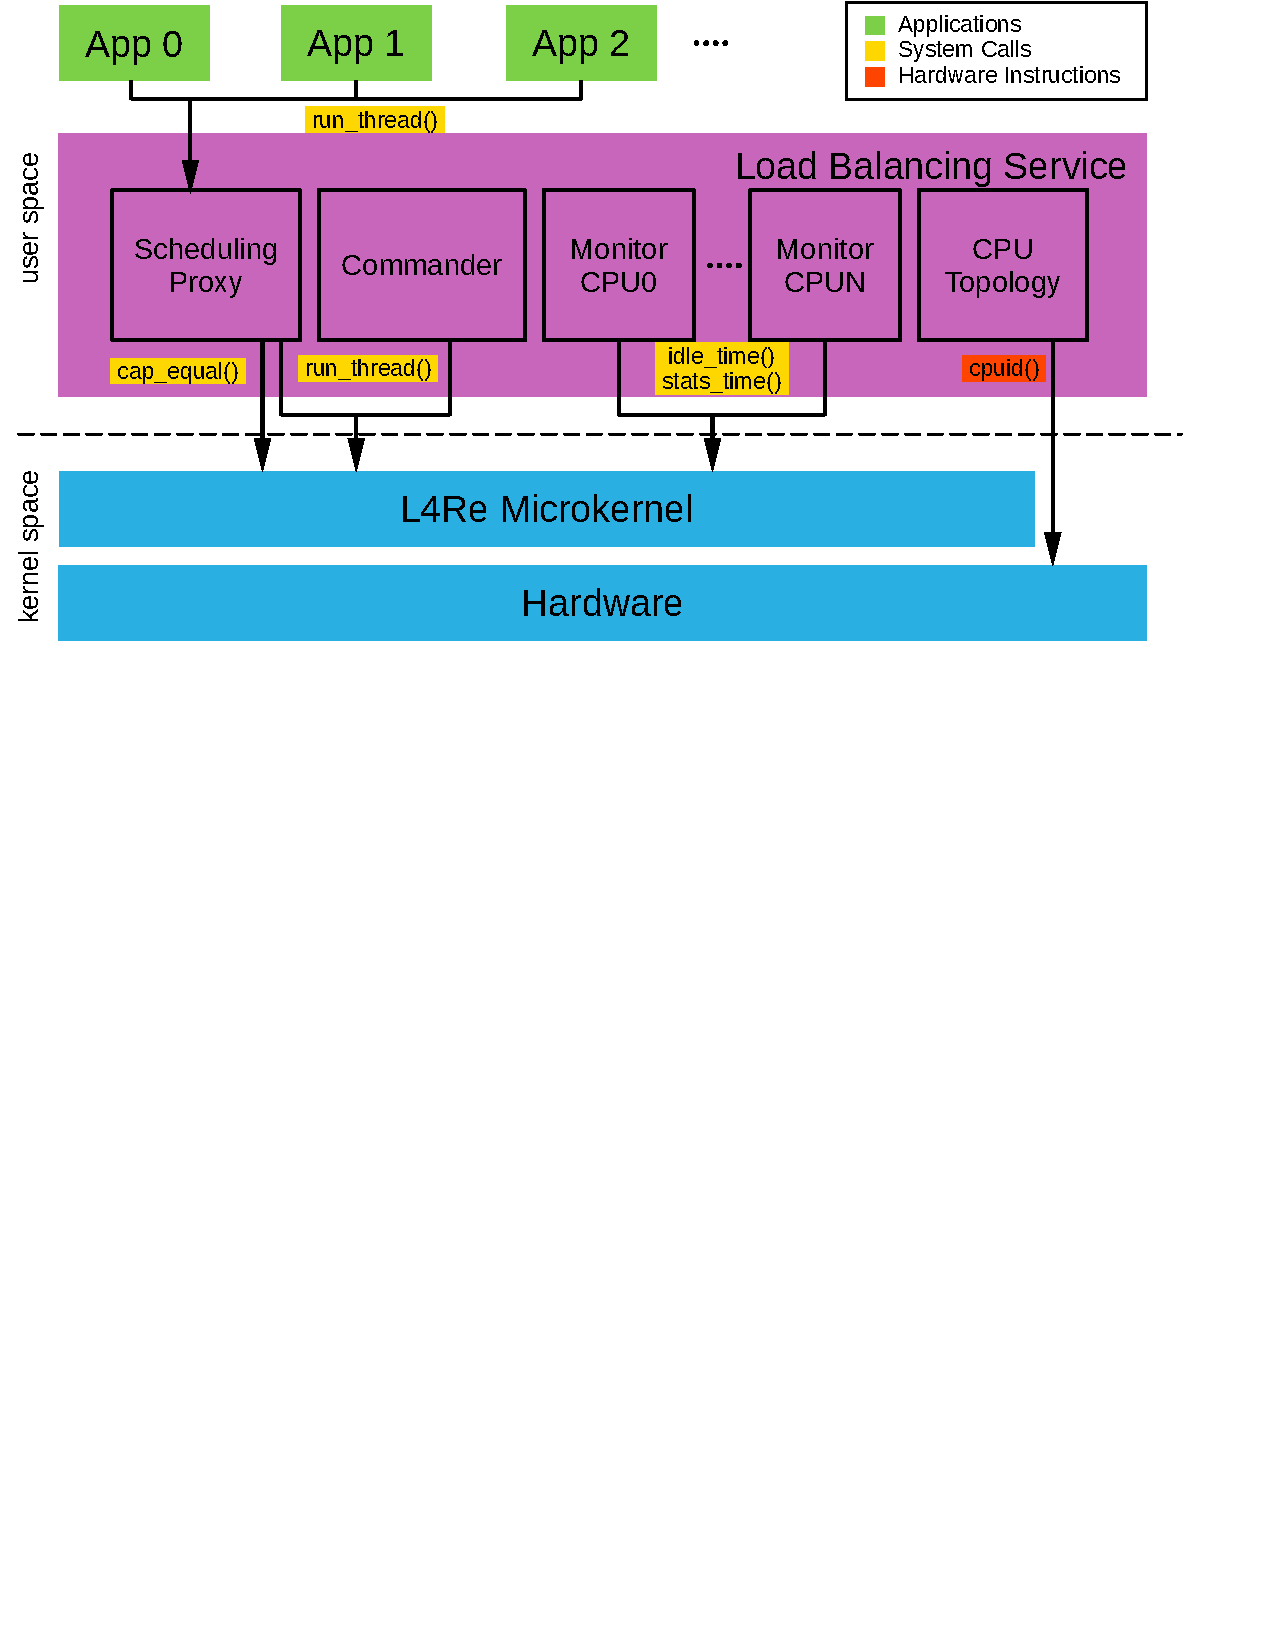
\includegraphics[trim={0 17.1cm 1.9cm 0}, clip, width=0.95\textwidth]{images/arch_overview_design.pdf}
	\caption{Architecture diagram at the design stage, showing the main components of the load balancing service and the communication between applications, the load balancer, and the kernel.}
	\label{fig:des:overview}
\end{figure}

The first component is a scheduling proxy that follows the L4Re proxy pattern (see Section~\ref{sec:proxy}) to receive scheduler calls like \texttt{run\_thread()} from the application to forward them to the actual kernel scheduler afterward.
During the interception, decisions can be made that enforce a given policy.

Second is the monitoring infrastructure consisting of one thread per CPU.
They track the runtime information of the idle thread and all regular scheduled threads on that CPU.

The commander is a thread that aggregates monitoring data and periodically triggers a rebalancing event.
During the rebalancing, overloaded and underloaded CPUs are identified, and migrations are ordered to bring the system back in balance.

Thread groups are the fourth and only component not visible in Figure~\ref{fig:des:overview}.
A thread group defines a CPU set that restricts members of that group to only run on dedicated CPUs allowed by the assigned CPU set.

The fifth component is the CPU topology, a structure that describes the topology of the hardware the load balancer observes.
In the case of non-uniform performance and structure of the CPUs, it retrieves information about processing speeds and location of hardware threads compared to cores, sockets, and further.

The whole design and implementation is based on the assumption that the underlying hardware architecture is x86.
Although the concepts would still suffice for other architectures, the concrete implementation would not work for individual components.

\section{Scheduling Proxy for Load Balancing}
\label{sec:des:proxy}

To appear as a scheduler instance, the load balancing proxy needs to implement all methods that the scheduler interface exposes.
The implemented functions can execute arbitrary policies as long as they adhere to the interface signature.
All calls of that interface except for \texttt{run\_thread} can be immediately forwarded to the scheduler of the scheduling proxy.
This does not necessarily need to be the kernel scheduler, as the proxy pattern allows layered scheduler instances on top of each other.

The entry point into the load balancing service is \texttt{run\_thread}.
This function is called by an application whenever it wants to run a specific thread with a set of scheduling parameters determining the thread's scheduling attributes.
It does not matter whether the thread is newly created or already exists.

The scheduling proxy shadows the threads and run queues currently in the system.
For this, it needs to compare the passed thread capability against all tracked capabilities to identify whether the thread is already being tracked.
If that is not be the case it is added to the bookkeeping structures.
Afterward, it will adapt all scheduling parameters according to its policy and forward the request to its designated scheduler.

\section{Monitoring the System State}
\label{sec:des:monitoring}

To make an informed migration decision, it is crucial to have information about the system state.
There are two system calls enabling this monitoring.
\begin{itemize}
	\item \texttt{L4::Scheduler::idle\_time()} is a call to the scheduler returning the total idle time of the CPU from which the request was made.
	\item \texttt{L4::Thread::stats\_time()} is taking a thread capability and returning the total runtime of the corresponding thread.
\end{itemize}
These methods allow identifying the load of a CPU and all threads currently tracked by the scheduling proxy.

A centralized approach checking every CPU and all threads of its run queue scales poorly with increasing CPU and thread counts; therefore, the design opts for a parallel approach.
For every CPU that was detected by the load balancer service, a designated monitoring thread (monitor) is spawned and pinned to this CPU.
It is responsible for periodically probing the idle thread's run time and state of the members of the local run queue.

Not only is it beneficial to have a run queue per CPU, but also the ready queue that only contains threads that are ready to run and, therefore, not blocked.
The scheduler interface does not provide a method like \texttt{get\_ready\_queue}.
This problem can be solved by extending the already existing \texttt{stats\_time()} call to not only return the runtime of the threads but also their thread state.
This call will be extended further in Section~\ref{sec:des:loba}.
Because the run queue needs to be iterated, it can be thereby annotated if a thread is currently ready or blocked.

\section{Commander Thread}
\label{sec:commander}

The commander thread (commander) is the central point of coordination for rebalancing decisions.
It collects all system information from the monitoring threads to make an informed migration decision.
This design falls into the category of centralized approaches for load balancing (see Section~\ref{sec:approaches}).
L4Re is built around the concept of strong isolation and the principle of least authority, or POLA for short.
Therefore, the system state information is distributed throughout multiple components that need to be collected separately, leading to a distributed system architecture.
Instead of having numerous instances access multiple sources at once, forcing complex behavior and access patterns, the design pivots to having one instance bundling multiple sources of information.
Three designs have been explored for aggregating monitoring information.

\subsection{Classic IPC.}

In L4Re, the IPC mechanism (see Section~\ref{sec:ipc}) is synchronous, so the commander would iterate through the monitoring threads.
This has the benefit of receiving up-to-date information from all CPUs and run queues.
However, the commander blocks for the whole time each monitor needs to retrieve the system state, resulting in poor scalability with growing CPU counts.
Additionally, the load balancer is a userland component, which means that every one of its threads can be preempted by other threads with higher priority.
This scenario is intended behavior, as a thread with higher priority should always be preferred by the system scheduler, but this could block the commander for an arbitrary amount of time when a monitor on a different CPU gets suspended.
At that point, the benefit of having up-to-date information from all CPUs does not hold anymore, as previously collected information will be outdated after blocking arbitrarily.

\subsection{Interrupt Notifications.}

To avoid iterating monitoring threads one after another but make use of having one monitor per CPU, the commander could be notified via interrupts.
Requesting the collection of all monitors at once and rebalancing when the final interrupt signals the return of the slowest monitor.
This approach parallelizes the monitoring process; hence, wall-clock time reduces from $\mathcal{O}(n)$ to $\mathcal{O}(1)$.
The drawback of this choice stems from most communication happening cross-CPU.
This assertion implies that for one request from the commander to a monitor and back, two IPIs are required (see Section~\ref{sec:cross-comm}), and excessive use of IPIs should be avoided at all costs.
Further, the problem of preempted monitors needs to be handled, for example, by bounding the waiting time of the commander with a timeout.
At that point this solution is more complex and costly than the previous approach.

\subsection{Asynchronous and Non-Blocking Coordination via Absolute Timeouts.}
\label{sec:abs-timeouts}

L4Re provides a primitive that allows a thread to not only sleep for a relative amount of time but also until an absolute system time is reached.
This mechanism allows the monitors and the commander to sleep until the next monitoring interval is reached.
The monitoring threads wake up first and retrieve the system state, and the commander sleeps for a fraction of the monitoring interval longer.
Upon waking up, it needs to be checked via timestamps to see if the monitors were able to update the system state in time to not read outdated information.
This approach combines the benefits of both previous solutions because an absolute timeout is implemented using efficient core-local IPC while also retaining the parallelism in monitoring.
This solution assumes a synchronized system clock for all participants, which is provided by the L4Re microkernel.

\paragraph{Key Insight.}
\label{sec:insight-prio}

The problem of load balancing threads getting preempted leads to an important discovery.
The load balancer cannot properly balance tracked threads that have a higher priority than the priority it is scheduled on itself.
This results from designing a scheduling component in userland, as the code does not run in kernel mode and is not only interruptible but also preemptible.
Therefore, the load balancer should obtain the highest priority possible, so the worst case would be round-robin scheduling with other threads of the same (maximum) priority.

\section{Load Balancing}
\label{sec:des:loba}

To be able to balance workload inside the system, a definition of load and, further, of over- and underload needs to be determined.
The intuitive solution would be to work with the current CPU utilization (from now on referred to as CPU load), which can be determined by the runtime of the CPU's idle thread.
This approach works well until the CPUs reach a load of 100\,\% or, inversely, an idle time of 0.
If ready threads start to accumulate faster on a CPU than they can be served, it is desirable to treat all threads fairly and move them to other CPUs that may also be at 100\% capacity but with shorter ready queues.

Thus, using CPU load as a one-dimensional balancing metric is insufficient to solve a multidimensional problem.
The USE (utilization, saturation, and errors) method, proposed by Brendan Gregg~\cite{use_method_gregg}, identifies utilization as just one dimension of performance.
Saturation needs to be regarded as well for CPU workloads, as it describes the pressure that accumulates on a CPU by growing run queue sizes.
Errors can be ignored in the scope of this work because USE was introduced in the context of distributed network systems, and CPUs do not drop instructions.

Linux employs a virtual runtime (see Section~\ref{sec:best-effort}) to capture utilization and saturation at once.
This method cannot be used to define CPU load either because L4Re is based on priorities and does not use time budgets for threads.

The metric used in this work builds upon the information of whether a thread was preempted during its time slice or gave up the CPU voluntarily.
Preemptions can happen either through a thread of higher priority becoming ready and replacing the previously running thread or the timer interrupt at the end of the time slice.  
Voluntarily yielding the CPU is considered everything that is not covered by preemption, for example, calling \texttt{yield()}, making an IPC call, or blocking through sleeping.
Capturing this information for every thread gives insight into how compute-demanding it was during its previous time slices.
Accumulating this metric for the whole run queue of a CPU strongly correlates with the CPU time consumed, but it also can outgrow 100\% CPU load.
This characteristic is important because threads that were compute-heavy in the past and are now suspended still add pressure to that CPU, although they do not receive any CPU time.
Of course, this metric can be tricked under special circumstances when threads would use a large amount of their time slice and then yield the CPU to seem computationally lightweight.
This behavior is a potential problem but not assumed as the average case.
Hence, the metric is able to capture utilization and saturation, making it more robust than just pure CPU load.
The metric derived from the tracked preemptions and used to determine the load of a CPU is called virtual load or \texttt{vload}.

The preemptions of a thread need to be collected for every thread tracked in the system.
This can again be solved by extending the already existing \texttt{stats\_time()} system call to additionally return the preemptions of a thread in addition to its blocked or ready state and its used CPU time.

\section{Thread Groups}
\label{sec:thread-groups}

Thread groups were created to solve the task of providing explicit scheduling groups for threads inside the system.
One example of a component that assumes separation of threads is the L4Re virtual machine monitor, UVMM.
When it creates multiple vCPUs, it is desirable to have them running on different physical CPUs.
Mostly because timesharing for vCPUs of the same VM does not make any sense, and busy-waiting primitives are used in virtual machines.
In addition to having vCPUs separated on hardware at all times, they are implemented as multiple threads.
The threads that make up one vCPU need to be placed on the same physical CPU at all times.

To employ a single source of truth, thread groups were introduced.
One unique group can be created per CPU scheduling set containing all the threads that were issued with the corresponding group's CPU set.
The member threads in a group are only allowed to run on the CPUs specified by the group's CPU set.
The layout of CPU sets is not restricted to any particular subset structure, so the number of possible thread groups is $2^n$ for $n$ available physical CPUs.
In practice, only a small subset of groups is used.
Additionally, the L4Re data type specifying a CPU set (\texttt{l4\_sched\_cpu\_set\_t}) does not allow all possible cases.

\begin{figure}[h]
	\centering
	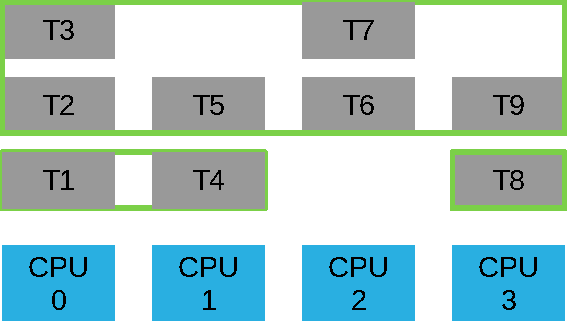
\includegraphics[width=0.6\textwidth]{images/thread_groups.pdf}
	\caption{Thread group example with four CPUs, nine threads (T), and three thread groups (green frames) limiting the placement of their threads to the CPUs they span. Thread group \{T1, T4\} on CPU0 and CPU1, group \{T2, T3, T5, T6, T7, T9\} on all CPUs, and group \{T8\} on CPU3.}
	\label{fig:thread-groups}
\end{figure}

If individual groups would experience poor performance, there is the option to reassign the physical CPUs that represent the available CPU sets to the groups.
The constraint that certain groups are not allowed to share physical CPUs during the reordering must not be violated.
Therefore, groups do not share physical CPUs with other groups; they are disjoint from in the originally assigned CPU set, and this remains true during reassignment as well.

The moment groups would have their CPU sets reassigned, applications that rely on thread pinning could have that assumption violated.
A countermeasure to this problem is the introduction of thread groups that represent pinned threads and do not have their CPU set reassigned.
This posed the problem of receiving the information if a thread should be pinned or not via the \texttt{run\_thread()} call.
One option would be to add a field to the scheduling parameters that are passed during the call.
In doing so, one would create severe ripple effects throughout the whole L4Re framework, as either a new scheduling parameter type would need to be created or all existing instances would require adaptation.
The approach chosen for this work was to add another \texttt{run\_thread\_pinned()} call to the scheduler interface, which passes a parameter if the thread should be pinned or not.

\section{Priority Translation}

The placement decision made during the handling of \texttt{run\_thread()} is just one policy enforced by the proxy; another can be to alternate the scheduling priority of a thread.
A scheduling proxy can be used to restrict or broaden the available priority band in any way.
Hence, the load balancer has the ability to move applications to low-priority, best-effort, or high-priority, real-time execution.
During the creation of the load balancer, a priority band can be assigned that then is used by the proxy to have threads end up only inside the specified priorities.

In the scope of this work two policies for priority translation were implemented from which a user can choose from during the creation of the load balancer.
When no strategy is specified, the default policy is chosen.

\paragraph{Cutoff.}

The default strategy is a cutoff applied to the resulting priority band.
If a thread is issued with a priority lower than the minimum, it is raised to the minimum.
Vice versa, the priority is lowered if the thread is issued with a priority higher than the maximum.
When the issued priority is inside the allowed priority band, no modification is made.

\paragraph{Priority Scaling.}

The second strategy scales the priority from the system's default priority band (0-255) to the specified range.
The relative position of the issued priority stays the same compared to the boundaries of the destination priority range. This preserves the relative priority differences within an application.

\medskip

Although both strategies may prove disadvantageous depending on the specific use case, the design allows for easy extension with additional policies tailored to future requirements.
Priority translation was not the focus of this thesis, so the two implemented strategies should be regarded as a default implementation rather than a central contribution.

\paragraph{Key Insight.}

L4Re defines its scheduling priorities as core-local.
This concept no longer holds the moment a thread needs to be migrated from one CPU to another.
Beforehand, a migration could only be issued by an application, which then needed to pass corresponding scheduling parameters with a given priority to the scheduler.
Therefore, the decision of what priority to advance with was left to the user.
To solve the problem of core-local priorities, they are assumed to be global for the load balancing component.

\section{CPU Topology}

The reading of the CPU topology is the main reason why this work relies on the x86 architecture, because it provides the \texttt{cpuid()} assembly instruction in userland.
Architectures such as ARM do not expose an equivalent instruction outside the kernel.
Retrieving the same topology information there would require extending the kernel itself and adding an interface through which userland could query the collected data, since userland has no direct means of reading it on its own.
\texttt{cpuid()} allows reading CPU-specific hardware information such as vendor identification, processor signature, feature flags, cache and TLB details, as well as power and thermal information~\cite{intel-cpuid}.
Tools like \texttt{lstopo} make use of most of this data to gain full insight into the hardware on which the operating system is executed.
For this work, the topology information alone is sufficient.

The design for reading CPU information is heavily inspired by an internal, non-public, existing L4Re userland module.
It reads the CPU topology to manage the separation of CPUs for applications that prohibit core sharing.
Because caches can be shared between multiple CPUs on the same physical core, a malicious thread could otherwise read cache information belonging to another application running on a CPU sharing that core.
To eliminate this threat, potentially affected applications require their threads to run on cores that are isolated and shared with no other application.

Evaluating the CPU information was simplified by reading all CPUs first and constructing the topology once afterward, rather than exploring a CPU and constructing part of the topology before reading the next one.

\subsection{CPU Performance Detection}
\label{sec:cpu-performance}

Not only is it beneficial to have insight into the CPU topology when hardware is asymmetric (see Section~\ref{sec:hetero-cpu-arch}), but also it is advantageous if the CPUs themselves are heterogeneous.
Distinguishing performance and efficiency cores is crucial, as they will behave differently under the same workload.

For the design in this work, an idea from the paper of Li and colleagues~\cite{faster-core-first} was adopted, where load balancing is made AMP-aware by scaling the compute power of each CPU based on its instructions executed per cycle.
By doing so, it breaks the heterogeneous hardware down to uniform processing, as the load of each CPU can be scaled by its processing speed.
Scaling CPU performance to obtain a uniform hardware abstraction works against the idea of having asymmetric CPUs in the first place, but this shows that not only is multiprocessor scheduling a non-trivial problem to solve, but it also gets even harder when underlying hardware is non-uniform.

The detection is done via microbenchmarks during the start phase of the load balancer.
For this one thread is spawned to each CPU measuring processing speed next to reading the CPU topology via \texttt{cpuid()}.
The compute performance of each CPU is then compared and scaled upwards relative to the slowest result.
The performance value is scaled in steps of 0.1.
Hence, a CPU scaled with 3.5 is three and a half times faster than the slowest CPU in the system.
To avoid unnecessary computation, the performance measurements are not done when the topology information returns that the system is uniform and therefore not composed of performance and efficiency cores.

Performance and efficiency cores are powerful in theory, but it is difficult to fully harness them as an operating system in practice.
Doing so requires sophisticated monitoring of the threads' behavior to classify them correctly, which is even more difficult in a microkernel and thus out of scope for this thesis.
Established operating systems like macOS, Windows, or Linux can make use of this kind of hardware because they can analyze their threads' behavior thoroughly.

\cleardoublepage

%%% Local Variables:
%%% TeX-master: "diplom"
%%% End:
